\documentclass[dvipdfmx]{jsarticle}
\usepackage[dvipdfmx]{graphicx}
\usepackage{amsmath, amssymb}
\usepackage{mathtools}
\usepackage{here}

\renewcommand{\thefigure}{\thesection.\arabic{figure}}
\setcounter{section}{4}
\setcounter{figure}{8}

\begin{document}

\section*{4.3 周波数選択性フェージングチャネルの容量}

ここでは,周波数選択性フェージングチャネルのシャノン容量について考察する.まず,時間不変の周波数選択性フェージングチャネルの容量を考える.この容量解析は,時間軸を周波数軸に置き換えたフラットフェージングチャネルの容量解析と同様である.次に,時間変動する周波数選択性フェージングチャネルの容量について考察する.

\section*{4.3.1 時不変チャネル}

図4.9に示すような周波数応答$H(f)$を持つ時不変チャネルを考える.チャネルが時不変である場合,一般的に送信機と受信機の両方で$H(f)$が既知であると仮定する.このチャネル知識の異なる仮定における時不変チャネルの容量は[18]で議論されている.

\begin{figure}[htbp]
\begin{center}
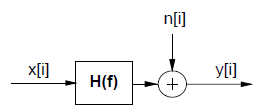
\includegraphics[width=0.5\linewidth]{spring_lec/wc4-3-1.png}
\end{center}
\caption{時不変の周波数選択性フェージングチャネル}
\end{figure}

まず,図4.10に示すように,$H(f)$がブロックフェージングで,周波数が帯域幅$B$のサブチャンネルに分割され,$H(f) = H_j$が各ブロックで一定であると仮定しよう.すると,周波数選択性フェージングチャネルは,$j$番目のチャネル上のSNR $|H_j|^2 P_j / (N_0 B)$と並列なAWGNチャネルのセットからなる.

この並列なセットのチャネル容量は,すべてのチャネルに最適に割り当てられた電力で各チャネルに関連するデータレートの合計である[5,6].

\begin{equation}\label{}
C = \sum_{\max P_j : \sum_j P_j \leq P} B \log_2 (1 + \frac{|H_j|^2 P_j}{N_0 B})
\tag{4.23}
\end{equation}

\noindent
これは,フラットフェージングチャネルの容量と最適な電力配分と同様であり,電力とデータレートは確率的な方法で時間と共に変化するのではなく,決定論的な方法で周波数と共に変化することに注意しなければならない.最適な電力配分は,フラットフェーディングの場合に使用したのと同じラグランジュ技法によって求められ,その結果,水充填電力配分(注水定理)が導かれる.

\begin{equation}
\frac{P_j}{P} =
\begin{dcases}
\frac{1}{\gamma_0} - \frac{1}{\gamma_j} & (\gamma_j \geq \gamma_0) \\
0 & (\gamma_j < \gamma_0)
\end{dcases}
\tag{4.24}
\end{equation}

\begin{figure}[htbp]
\begin{center}
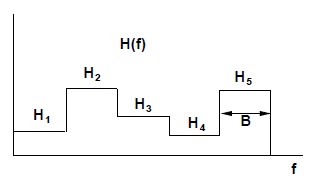
\includegraphics[width=0.6\linewidth]{./spring_lec/wc4-3-2.png}
\end{center}
\caption{ブロック周波数選択性フェージング}
\end{figure}

\noindent
あるカットオフ値$\gamma_0$に対して,$\gamma_j = |H_j|^2 P / (N_0 B)$は,j番目のチャネルに電力量全体が割り当てられたと仮定した場合のSNRである.この最適な電力配分を図4.11に示す.カットオフ値は電力適応の式を電力制約に代入して得られるので,$\gamma_0 $は以下を満たす必要がある.

\begin{equation}
    \sum_j (\frac{1}{\gamma_0} - \frac{1}{\gamma_j}) = 1
\tag{4.25}
\end{equation}

\noindent
このとき,容量は次のようになる.

\begin{equation}
    C = \sum_{j:\gamma_j \geq \gamma_0} B \log_2 (\gamma_j / \gamma_0)
\tag{4.26}
\end{equation}

\noindent
この容量は,各サブチャネルで異なるデータレートとパワーで送信することで実現される.マルチキャリア変調は,12章で詳しく説明するように,アダプティブ・ローディングで同じ技術を使用している.

\begin{figure}[htbp]
\begin{center}
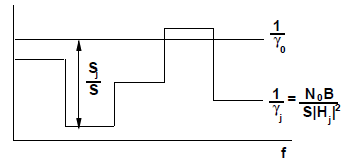
\includegraphics[width=0.6\linewidth]{./spring_lec/wc4-3-3.png}
\end{center}
\caption{ブロック周波数選択性フェージングにおける水充填}
\end{figure}

$H(f)$が連続的な場合,電力制約$P$の下での容量はブロックフェージングチャネルの場合と同様であり,チャネル容量が次式で与えられることを示すには,いくらかの数学的な複雑さが必要である.

\begin{equation}\label{}
    C = \max_{P(f):\int P(f) df \leq P} \int \log_2 (1 + \frac{|H_j|^2 P(f)}{N_0} df)
\tag{4.27}
\end{equation}

\noindent
積分内部の式は,電力配分$P(f)$とチャネル利得$|H(f)|^2$による帯域幅$df$上の与えられた周波数$f$に関連する容量の増分と考えることができる.この結果は,チャネル$h(t)$の Karhunen-Loeve展開を使用して,並列独立チャネルの等価セットを作成することで正式に証明される [5, 8.5章]を参照.別の証明として,離散フーリエ変換(DFT) [12]を用いてチャネルを並列集合に分解する方法もある.同じ前提が,12.4章で説明するマルチキャリア変調の離散実装で使用される.

(4.27)を最大化する周波数に対する電力配分$P(f)$はラグランジュ技法によって求められる.その結果,最適な電力配分は周波数に渡って注水定理に従う.

\begin{equation}
\frac{P(f)}{P} =
\begin{dcases}
\frac{1}{\gamma_0} - \frac{1}{\gamma (f)} & (\gamma (f) \geq \gamma_0) \\
0 & (\gamma (f) < \gamma_0)
\end{dcases}
\tag{4.28}
\end{equation}

\noindent
この結果,チャネル容量は
\begin{equation}\label{}
C = \int_{f:\gamma (f) \geq \gamma_0} \log_2 (\gamma(f) / \gamma_0) df
\tag{4.29}
\end{equation}
と表される.

\section*{4.3.2 時変チャネル}

\noindent
時間的に変化する周波数選択性フェージングチャネルは,$H(f) = H(f, i)$,すなわちチャネルが周波数と時間の両方で変化することを除いて,図4.9に示すモデルと同様である.時間的に変化する周波数選択性フェージングチャネルは,送受信機で瞬間的なチャネル$H(f, i)$が完全に分かっていても,自己干渉(ISI)のランダムな影響により容量を決定することが困難である.送受信機側情報がある場合,最適な適応方式は,過去の送信ビット列に対するチャネルの影響と,これらのビットに起因するISIが将来の送信にどのように影響するかを考慮しなければならない[30].時間変動する周波数選択性フェージングチャネルの容量は一般に未知であるが,上・下限値や制限式は存在する[30, 31].

図4.12に示すように,関心のあるチャネル帯域幅$B$を取り,チャネルコヒーレンス帯域幅$B_c$の大きさのサブチャネルに分割することによって,時間変動周波数選択性フェージングにおけるチャネル容量を近似的に求めることができる.そして,得られた各サブチャネルは独立で時変であり,j番目のサブチャネルで$H(f, i)= H_j[i]$のフラット・フェージングであると仮定する.

この仮定のもと,総電力制約$P$に従い,各サブチャネルに割り当てる平均電力$\overline{P}_j$に基づいて,これらフラットフェージングサブチャネルそれぞれの容量を求める.チャネルは独立しているので,総チャネル容量は,時間と周波数の両方で平均化された,総平均電力制約に従う個々の狭帯域フラットフェージングチャネルの容量の和にちょうど等しくなり,

\begin{equation}\label{}
C = \max_{{\overline{P}_j}:\sum_j \overline{P}_j \leq \overline{P}} \sum_j C_j (\overline{P}_j)
\tag{4.30}
\end{equation}

\noindent
ここで,$C_j(\overline{P}_j)$は平均電力$P_j$と帯域幅$B_c$のフラットフェージングサブチャネルの容量で,異なるサイド情報および電力配分方針の下でのシャノン容量について(4.13), (4.4), (4.18), または(4.22)で与えられている.また,受信機のみがサイド情報を持つ場合の容量対停電として$C_j(\overline{S}_j)$を定義することができる.

ここでは,完全な送受信チャネルCSIを仮定したシャノン容量に注目する.なぜなら,これは他のあらゆる側面情報の仮定や最適でない電力配分戦略の下で上界する容量だからである.サブチャネルあたりの平均電力を固定すると,最適電力適応は注水定理に従うことが分かっている.また,各サブチャネルに割り当てられる最適な平均電力も注水定理に従うはずで,より良いサブチャネルにはより多くの平均電力が割り当てられると予想される.したがって,最適な電力配分は,時間と周波数の両方において2次元の注水になると予想される.次に,この最適な2次元注水とそれに対応するシャノン容量を求める.

$\underline{\gamma_j}[i] = |H_j[i]|^2 \overline{P} / (N_0 B)$を,その時間および周波数に総電力$P$が割り当てられたと仮定した場合の時間$i$における$j$番目のサブチャネルの瞬時SNRと定義する.電力$P_j(\gamma_j)$は$\gamma_j[i]$に応じて変化することを許容する.完全な送受信機CSIを持つシャノン容量は,時間($\gamma_j[i] = \gamma_j$で表される)と周波数(サブチャネルインデックス$j$で表される)の両方に対して電力適応を最適化することによって与えられる.

\begin{equation}\label{}
C = \max_{P_j(\gamma_j):\sum_j \int_{0}^{\infty}P_j (\gamma_j) p(\gamma_j) d_{\gamma_j} \leq \overline{P}} \sum_j \int_{0}^{\infty} B_c \log_2 (1 + \frac{P_j (\gamma_j) \gamma_j}{\overline{P}}) p(\gamma_j) d\gamma_j
\tag{4.31}
\end{equation}

\noindent
最適電力配分$P_j(\gamma_j)$を見つけるために,ラグランジアンを形成して,

\begin{equation}\label{}
J(P_j(\gamma_j)) = \sum_j \int_{0}^{\infty} B_c \log_2 (1 + \frac{P_j (\gamma_j) \gamma_j}{\overline{P}}) p(\gamma_j) d_{\gamma_j} - \lambda \sum_j \int_0^{\infty} P_j (\gamma_j) p(\gamma_j)d\gamma_j
\tag{4.32}
\end{equation}

\noindent
(4.32)は,サブチャネルの総和によって周波数の次元が追加されていることを除けば,フラットフェージングチャネルのラグランジアン(4.10)と同様であることに注意されたい.ラグランジアンを微分し,この微分をゼロとすることで,与えられたサブチャネルと関連するSNR以外のすべての項が排除される.

\begin{equation}\label{}
\frac{\partial{J}(P_j(\gamma_j))}{\partial{P_j}(\gamma_j)} = \left[(\frac{B / \ln(2)}{1 + \gamma_j P(\gamma_j) / \overline{P}}) \frac{\gamma_j}{\overline{P}} - \lambda \right] p(\gamma_j) = 0
\tag{4.33}
\end{equation}

\noindent
$P_j(\gamma_j)$を解くと,フラットフェーディングの場合と同じ注水が得られる.

\begin{equation}
    \frac{P_j(\gamma_j)}{\overline{P}} =
    \begin{dcases}
    \frac{1}{\gamma_0} - \frac{1}{\gamma_j} & (\gamma_j \geq \gamma_0) \\
    0 & (\gamma_j < \gamma_0)
    \end{dcases}
\tag{4.34}
\end{equation}

\noindent
ここで,カットオフ値$\gamma_0$は,時間および周波数の両方にわたる総電力制約から得られる.

\begin{equation}\label{}
\sum_j \int_{0}^{\infty} p_j (\gamma) p_j (\gamma) d\gamma_j = \overline{P}
\tag{4.35}
\end{equation}

\noindent
したがって,最適な電力配分(4.34)は,共通のカットオフ値$\gamma_0$を持つ2次元の注水となる.制約条件(4.35)を$P$で割り,最適電力配分 (4.34)に代入すると,$\gamma_0$ は以下を満たす必要があることがわかる.

\begin{equation}\label{}
    \sum_j \int_{0}^{\infty} \left(\frac{1}{\gamma_0} - \frac{1}{\gamma_j}\right) p_j (\gamma) d\gamma_j = 1
\tag{4.36}
\end{equation}

\noindent
2次元の注水では,すべてのサブチャネルのカットオフ値が同じであることは興味深いことである.これは,サブチャネルのフェージング分布や平均フェードパワーが異なっていても,瞬時SNRが共通のカットオフ値$\gamma_0$を下回ると,全てのサブチャネルが送信を中断することを意味する.最適電力配分(4.35)を容量式(4.31)に代入すると,次のようになる.

\begin{equation}\label{}
    C = \sum_j \int_{0}^{\infty} B_c \log_2 \left(\frac{\gamma_j}{\gamma_0}\right) p_j (\gamma) d\gamma_j
\tag{4.37}
\end{equation}

\end{document}